\begin{frame}[c]{Comunicación USB 2.0 para sistema científicos implementados en FPGA}
	\centering
	\begin{tikzpicture}[scale=.8,transform shape,>=latex]
		\node[bloque](pc){PC};
		\node[bloque](adq)[right =1.3 of pc]{Sistema de adquisicíon basado en FPGA};
		\node[bloque](sens)[right=1.3 of adq]{Sensor para datos científicos};
		\draw[<->,double]([yshift=10]pc.east) -- node [above]{Datos} ([yshift=10]adq.west);
		\draw[<->,double]([yshift=-10]pc.east) -- node [above]{Control} ([yshift=-10]adq.west);				
		\draw[<->,double]([yshift=10]adq.east) -- node [above]{Datos} ([yshift=10]sens.west);
		\draw[<->,double]([yshift=-10]adq.east) -- node [above]{Control} ([yshift=-10]sens.west);
	\end{tikzpicture}
	\begin{itemize}
		\item Los avances tecnológicos permiten el desarrollo de nuevos sensores.
		\item Estos sensores producen una gran cantidad de datos.
		\item Las ventajas que presentan los FPGA los convierte en dispositivos interesantes para la adquisición de los datos.
		\item La PC posibilita el procesamiento y análisis de datos.
		\item Se hace necesaria una comunicación veloz y eficaz entre la PC y el FPGA.
	\end{itemize}
\end{frame}

\begin{frame}{Selección del protocolo de comunicación}
	\begin{columns}
		\begin{column}{.3\textwidth}
			\centering 
			Ethernet\\
			\vspace{1mm}
			\centering 
			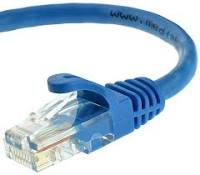
\includegraphics[height=.18\textheight]{ethernet}
		\end{column}
		\begin{column}{.3\textwidth}
			\centering
			Wi-Fi\\
			\vspace{1mm}
			\centering 
			
\includegraphics[height=.18\textheight]{wifi}
		\end{column}
		\begin{column}{.3\textwidth}
			\centering
			USB\\
			\vspace{1mm}
			\centering
			
\includegraphics[height=.18\textheight]{usb20}
		\end{column}
	\end{columns}
	\action<1>{
		\begin{columns}[t]
			\begin{column}{.32\textwidth}
				\begin{itemize}
					\item Gran ancho de banda (1 Gbps)
					\item Destinado a redes de PC
					\item Requiere infraestructura adicional
				\end{itemize}
			\end{column}
			\begin{column}{.32\textwidth}
				\begin{itemize}
					\item Buen ancho de banda (600 Mbps)
					\item Redes inalámbricas
					\item Comunicación inestable
				\end{itemize}
			\end{column}
			\begin{column}{.32\textwidth}
				\begin{itemize}
					\item Buen ancho de banda (480 Mbps)
					\item Destinado a periféricos
				\end{itemize}
			\end{column}
		\end{columns}}
	\action<2>{\vspace{-1.5cm}
			\centering \large{USB 2.0 resulta la mejor alternativa para comunicar periféricos a una PC sin comprometer funcionalidades importantes.\\}}
\end{frame}